\documentclass[pdf]{beamer}
\usetheme{Madrid} % You can change this to other themes like Madrid, Copenhagen, etc.
\usecolortheme{default}
\usepackage{tabularx}
\usepackage{lscape}
\usepackage{graphicx}
\usepackage{tikz}\usetikzlibrary{arrows.meta,calc} %library tikz
% Packages for math and symbols
\usepackage{amsmath, amssymb}
\usepackage{graphicx} % For including images if needed
\usepackage[utf8]{inputenc}

% Title slide information
\title[Classification of 2 lattices]{The Pentagonal Number Theorem and classification of two dimensional lattices}


\author{Tri Nguyen}


\begin{document}

% Title Slide
\begin{frame}
    \titlepage
\end{frame}

% Outline Slide
\begin{frame}{Outline}
    \tableofcontents
\end{frame}

\section{Introduction}
\subsection{Partition of a positive number $n$}
\begin{frame}{Warm-up problem}
    \begin{center}
        \textit{Given a positive number $n$, how many ways can we write $n$ in the form}
        \[a_1+a_2+\ldots+a_k?\]
    \end{center}
\end{frame}

\begin{frame}{Warm-up problem}
    There are in total $2^{n-1}$ of them, however, there are a lot of repetitions.
    \begin{table}
        \begin{tabular}{l  c  c  c  c }
            $n$ & 1 & 2   & 3     \\
            \hline\pause
                & 1 & 2   & 3     \\
                &   & 1+1 & 1+2   \\
                &   &     & 2+1   \\
                &   &     & 1+1+1
        \end{tabular}
        \caption{Initial partitions}
    \end{table}
\end{frame}

\begin{frame}{Warm-up problem}
    There are in total $2^{n-1}$ of them, however, there are a lot of repetitions.
    \begin{table}
        \begin{tabular}{l  c  c  c  c }
            $n$ & 1 & 2   & 3                    \\
            \hline\pause
                & 1 & 2   & 3                    \\
                &   & 1+1 & \textcolor{red}{1+2} \\
                &   &     & \textcolor{red}{2+1} \\
                &   &     & 1+1+1
        \end{tabular}
        \caption{Counting order-sensitive partitions}
    \end{table}\pause
    So you will get more and more repetitions listing this way. For example:
    \begin{align*}
        4 & = 1+1+1+1                                                                  \\
          & = \textcolor{red}{2+1+1} = \textcolor{red}{1+2+1} = \textcolor{red}{1+1+2} \\
          & = 2+2                                                                      \\
          & = \textcolor{blue}{3+1} = \textcolor{blue}{1+3}
    \end{align*}
\end{frame}

\begin{frame}{Partition}
    We don't want to over-count the number of "partitions", so we will restrict ourselves to just the ways we can write the number as a sum of positive integers, up to permutation. \pause
    \begin{block}{Partition}
        Given a positive integer $n$, we call a \textit{partition} of $n$ a representation of $n$ as a sum of positive integers, not taking into account the order of summands. We denote the number of partitions of $n$ by $p(n)$.
    \end{block} \pause
    So in the above examples, we have a few first values of $p(n)$.
    \begin{table}
        \begin{tabular}{l  | c | c | c | c | c | c | }
            $n$    & 1 & 2 & 3 & 4 & 5 & 6  \\
            \hline\pause
            $p(n)$ & 1 & 2 & 3 & 5 & 7 & 12
        \end{tabular}
        \caption{First few values of $p(n)$}
    \end{table}
\end{frame}

\begin{frame}{Euler's first formulae}
    Euler came up with the following generating function for $p(n)$
    \begin{block}{Theorem 1}
        We have the following identity
        \[(1+x+x^2+\ldots)(1+x^2+x^4+\ldots)(1+x^3+x^6+\ldots)(\ldots) = \sum p(n)x^n\]
    \end{block}
    \begin{proof}
        This is just combinatorics, we actually counts the number smaller than $n$ that appears the partition.
    \end{proof}
    A similar method can be used to count the number of partitions that contains a specific set of given number.
\end{frame}
\begin{frame}{Problems?}
    This method is very slow if one wants to compute $p(n)$ explicitly for $n$ larges.

    A programme in \textit{Mathematica} following this method takes around 50s to compute the first fifty values of $p(n)$.
\end{frame}
\subsection{Pentagonal number theorem}
\begin{frame}{A faster method}
    \begin{block}{Ring of formal series}
        Let
        \[\mathfrak{U} = \left\lbrace 1+a_1x+a_2x^2+\ldots = \sum_{\ge 0} a_nx^n\right\rbrace\]
        Then we can define a multiplication by
        \[(1+a_1x+a_2x^2+\ldots)(1+b_1x+b_2x^2+\ldots) =1+c_1x+c_2x^2+\ldots\]
        where $c_k = a_k + a_{k-1}b_1+\ldots+b_k$
    \end{block}
\end{frame}
\begin{frame}{A faster method}
    \begin{block}{Theorem 2}
        The set $\mathfrak{U}$ with this product forms a group.
    \end{block}
    \begin{proof}
        Left to the audiences =)).
    \end{proof}
    In particular, we have that
    \[\dfrac{1}{1-x^k} = \sum_{n \ge 0} x^{nk} = 1+ x^k+x^{2k}+\ldots\]
\end{frame}
\begin{frame}{A faster method}
    \begin{block}{Theorem 3}
        We have the following generating function for $p(n)$
        \[
            \dfrac{1}{\prod_{k \ge 1} (1-x^k)} = \sum_{n \ge 1}p(n)x^n
        \]
    \end{block}\pause
    \begin{proof}
        This follows from theorem 1 by taking the inverses of the series on the left hand sides.
    \end{proof}
\end{frame}
\begin{frame}{The pentagonal number theorem}
    Euler hoped to find a pattern that emerges from the denominator on the left hand side. He did that by multiplying everything and get the following
    \[\prod_{k \ge 1} (1-x^k) = 1-x-x^2+x^5+x^7-x^{12}-x^{15}+x^{22}+x^{26}-x^{35}-x^{40}+\ldots\]
    \pause
    Note that we obviously have
    \[(1-x-x^2+x^5+x^7-x^{12}-\ldots)(1+p(1)x+p(2)x^2+p(3)x^3+\ldots)=1\]\pause
    So we have a recurrence relation
    \[p(n)-p(n-1)-p(n-2)+p(n-5)+p(n-7)-p(n-12)-p(n-15)+...=0\]
    Using this relation, it is much faster to compute the partition number.
\end{frame}
\begin{frame}{Why Pentagonal?}
    If you list the exponents, you get a sequence of number
    \[1, 2,5,7,12,15,22,26,35,40,\ldots\]\pause
    The subsequence of number at the odd positions is
    \[1, 5, 12, 22,35,\ldots \]\pause
    All the terms showed up here are the pentagonal number! In particular, they are given by the formulae
    \[ n = \dfrac{k(3k-1)}{2}, \quad k \ge 1\]

\end{frame}
\begin{frame}{Why Pentagonal}
    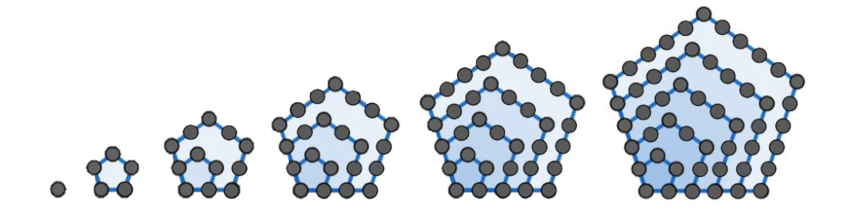
\includegraphics{The first six pentagonal number}
\end{frame}
\begin{frame}{Pentagonal number theorem}
    It turns our that the numbers at even positions is also given by pentagonal number formula, with oppositive sig
    \[n = \dfrac{k(3k-1)}{2}, \quad k \le -1\]
    So  Euler conjectured that
    \begin{block}{Pentagonal Number theorem}
        \[\prod_{k \ge 1} (1-x^k) = \sum_{k=-\infty}^\infty (-1)^kx^{\frac{k(3k-1)}{2}}\]
    \end{block}\pause
    This is later proved algebraically by Euler in 1750 and again by Franklin in 1881.
\end{frame}
\section{Modular forms}
\subsection{Elliptic integral}
\begin{frame}{Length of ellipse}
    We start with an old problem: \textit{How can we compute the perimeter of an ellipse?}
    \pause
    We consider the ellipse of the form
    \[\dfrac{x^2}{a^2}+\dfrac{y^2}{b^2}=1\]
    We know from calculus that the total length can be computed by
    \[\int\sqrt{(dx)^2+(dy)^2}= \sqrt{1+\left(\dfrac{dy}{dx}\right)}^2dx \]
\end{frame}
\begin{frame}{Length of an ellipse}
    Solve for the equation of ellipse in term of $y$, we get
    \[y = b\sqrt{1-\frac{x^2}{a^2}}\]
    which implies that
    the total length of an ellipse is
    \[4a \int_0^1 \sqrt{\dfrac{1-k^2t^2}{1-t^2}}dt = 4\int_0^1 \dfrac{1-k^2t^2}{\sqrt{(1-t^2)(1-k^2t^2)}}dt \] \pause%= 4\int_0^1 R(t,\sqrt{(1-t^2)(1-k^2t^2)}\] \pause
    where $k = \sqrt{\dfrac{a^2-b^2}{b^2}}$.

    For $k =0$, this is just the perimeter of the circle.  The general case is called \textit{elliptic integral}.

\end{frame}
\begin{frame}{A case study of Gauss}
    Gauss essentially tried to compute the elliptic integral by looking at the
    following integral
    \[F(x) = \displaystyle\int_0^x\dfrac{1}{\sqrt{1-z^4}}dz\]
    Mimicking the case for the integral
    \[ \int_0^x\dfrac{1}{\sqrt{1-z^2}}dz = \sin^{-1}(x)\]
    Gauss tried to find an inverse function of $F$. This inversion is called \textit{elliptic functions}.
\end{frame}
\begin{frame}{Weierstrass $\wp$ functions}
    Abel, and later Weierstrass, created an elliptic functions from scratch using the lattice.
    \begin{block}{Lattice}
        A lattice $L \subset \mathbb{R}^2$ is a set of the form
        \[L = \mathbb{Z}e_1\oplus\mathbb{Z}e_2\]
        where $e_1,e_2$ are linearly independent over $\mathbb{R}$.
    \end{block}
\end{frame}
\begin{frame}{Weierstrass $\wp$ functions}
    \begin{figure}[h]
        \centering
        \resizebox{70mm}{70mm}{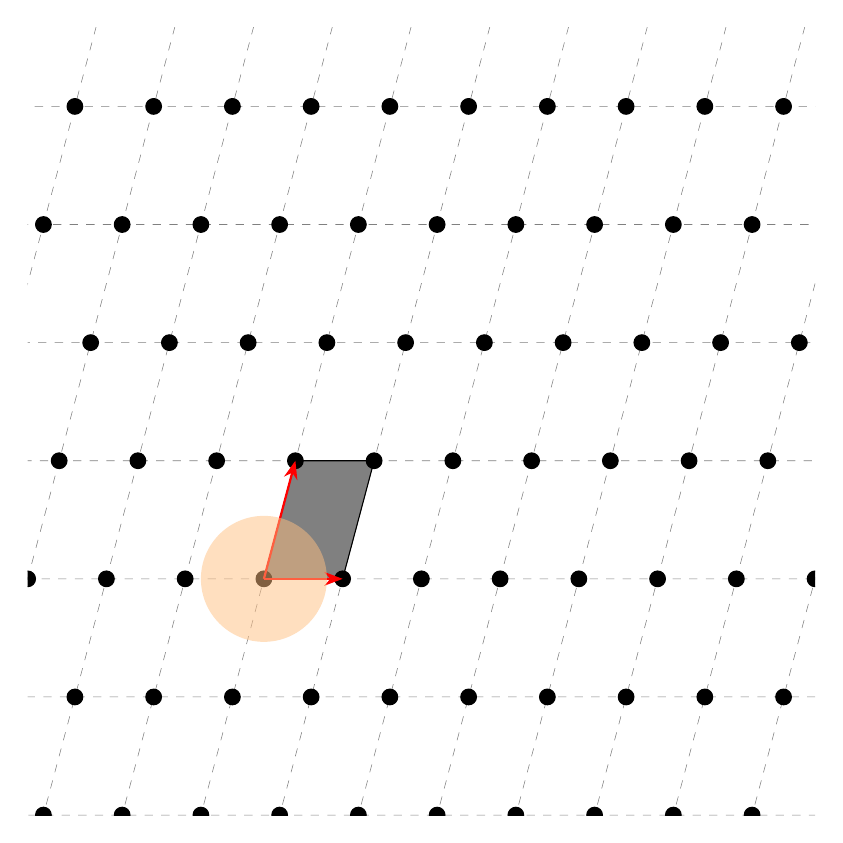
\begin{tikzpicture}
                \begin{scope}
                    \clip (0,0) rectangle (10cm,10cm); % Clips the picture...
                    \pgftransformcm{1}{0}{0.4}{1.5}{\pgfpoint{3cm}{3cm}} % Adjusted transformation matrix for less skew

                    \draw[style=help lines,dashed] (-14,-14) grid[step=1cm] (14,14); % Draws a grid in the new coordinates
                    \filldraw[fill=gray, draw=black] (0,0) rectangle (1,1); % Puts the shaded rectangle
                    \foreach \x in {-7,-6,...,7}{                           % Two indices running over each
                            \foreach \y in {-7,-6,...,7}{                       % node on the grid we have drawn 
                                    \node[draw,circle,inner sep=2pt,fill] at (\x,\y) {}; % Places a dot at those points
                                }
                        }
                    % Draw the vector from (0,0) to (1,0) in the transformed coordinate system
                    \draw[red, -Stealth, thick] (0,0) -- (1,0); % Vector from (0,0) to (1,0)
                    \draw[red, -Stealth, thick] (0,0) -- (0,1); % Vector from (0,0) to (0,1)

                \end{scope}
                % Place the circle at the lowest-left vertex (3,3) in the original coordinate system
                \fill[orange!50,semitransparent] (3,3) circle (.8cm); % Radius is 1.3cm to contain the shorter edge
            \end{tikzpicture}}
        \caption{Example of a lattice}
        \label{fig:example}
    \end{figure}
\end{frame}
\begin{frame}{Weierstrass $\wp$ functions}
    Weierstrass defined his function as
    \[\wp(z) = \dfrac{1}{z^2}+ \sum_{m,n \ne 0}\left(\dfrac{1}{(z-m\omega_1-n\omega_2)^2} -\dfrac{1}{(m\omega_1+n\omega_2)^2}\right)\]
    This function is holomorphic and doubly periodic.
    \pause
    Differentiating both sides yields another elliptic functions
    \[\wp'(z) = -2 \sum_{m,n}\dfrac{1}{(z-m\omega_1-n\omega_2)^3}\]
\end{frame}
\begin{frame}{Weierstrass $\wp$ functions}
    \begin{block}{Theorem : Doubly periodic functions with prescribed periods}
        Every doubly periodic function with periods $\omega_1,\omega_2$ can be written uniquely in the form
        \[R_1(\wp(z))+ R_2(\wp(z))\wp'(z).\]
        In other words, any doubly periodic function with periods $\omega_i$ is an element of the function field $\mathbb{C}(\wp,\wp')$
    \end{block}
    In particular, there are not many double periodic functions.
\end{frame}
\begin{frame}{Weierstrass $\wp$ functions}
    \begin{block}{Theorem }
        We have
        \[(\wp'(z))^2 = 4\wp(z)^3-g_2\wp(z)-g_3\]
    \end{block}
\end{frame}
\subsection{The modular picture}
\begin{frame}{Classification of lattices}
    Starting with the problem on the arc length of ellipse, we come up with the notion of lattices and elliptic functions. Do we know all the possible "lattice shape"?\vspace{3em}

    \pause
    \textbf{Answer:} Up to maginifcation, rotation and change of basis, the answer is yes.
\end{frame}
\begin{frame}{Fundamental domain}
    Up to rorations and magnifications, we can reduce a lattice
    \[L = \mathbb{Z}\omega_1 \oplus \mathbb{Z}\omega_2\]
    to a lattice of the form
    \[L_z = \mathbb{Z}z\oplus\mathbb{Z}, \quad \Im(z)>0\]
    So the upper half-plane parametrizes the 2 dimensional lattices.
    \begin{block}{Classification of unit lattices}
        The map $z \mapsto \mathbb{Z}z\oplus\mathbb{Z}$ induces a bijection
        \[\text{SL}_2(\mathbb{Z}) \backslash\mathbb{H} \cong \left\lbrace \text{ lattices}\right\rbrace/\mathbb{C^\times}\]
    \end{block}

\end{frame}
\begin{frame}{Fundamental domain}
    So we reduce to study the space of lattices by looking the action of $\text{SL}_2(\mathbb{Z})$ on the upper half plane. Geometrically, the domain is given by
    \[\mathfrak{D} = \left\lbrace z=x+iy \in \mathbb{H}: |z| \ge 1,-1/2 \le x \le 1/2 \right\rbrace \],
    \pause
    \[
        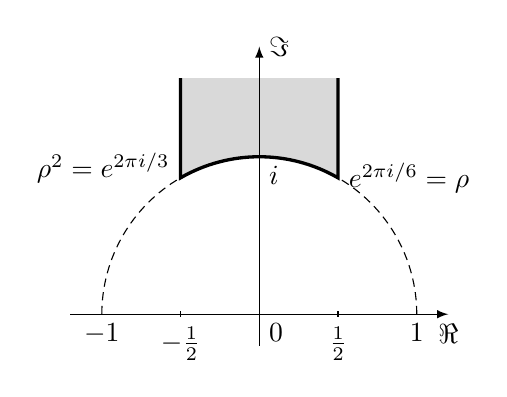
\begin{tikzpicture}[scale=2]
            \draw[densely dashed] (1,0) arc (0:60:1) (-1,0) arc (180:120:1);
            \draw[very thick, fill=gray!30] (.5,1.5) --node[right, pos=1]{$e^{2\pi i/6}=\rho$} (60:1) arc (60:120:1)
            --node[left, pos=.1]{$\rho^2=e^{2\pi i/3}$} (-.5,1.5);
            \draw[-latex] (-1.2,0) -- (1.2,0)node[below]{$\Re$};
            \draw[-latex] (0,-.2) -- (0,1.7)node[right]{$\Im$};
            \path(-1,0) --node[below, pos=0]{$-1$}node[below right, pos=.5]{0}node[below, pos=1]{1} (1,0)
            (0,1)node[below right]{$i$};
            \draw(-.5,.02)--(-.5,-.02)node[below]{$-\frac{1}{2}$}(.5,.02)--(.5,-.02)node[below]{$\frac{1}{2}$};
        \end{tikzpicture}\]
\end{frame}
\begin{frame}{A brief look at modular forms}
    \textbf{Goal:} we have to assign each point $z \in \mathfrak{D}$ a number $j(z)$ such that $j$ detects the $z$ corresponding to distinct lattices. \pause
    \begin{block}{Generators of $\text{SL}_2(\mathbb{Z})$}
        As a group,  $\text{SL}_2(\mathbb{Z})$ is generated by two elements
        \[S = \begin{bmatrix} 0 & -1 \\ 1 & 0 \end{bmatrix}, \quad T=\begin{bmatrix} 1 & 1 \\ 0 & 1 \end{bmatrix}\]
    \end{block}\pause
    So we are after a function $j \colon \mathbb{H} \to \mathbb{C}$ such that
    \[j(Sz)  = j(Tz) = j(z)\]
\end{frame}
\begin{frame}{A brief look at modular forms}
    If $g(z)$ is a holomorphic function on the unit disk, then $g(e^{2i\pi\tau})$ is a holomorphic function over the upper half plane and have a period $p=1$. So for each holomophic function on the unit disk, we get a candidate. The problem is to find a function $f(\tau)= g(e^{2i\pi\eta})$ such that
    \[f(\tau) = f\left(\dfrac{1}{-\tau}\right)\]
    We have the \textit{Eisenstein series} defined as
    \[g_4(\tau) = 60\sum_{m,n \ne 0} \dfrac{1}{(m\tau+n)^4}\]
    and
    \[g_6(\tau) = 140\sum_{m,n \ne 0} \dfrac{1}{(m\tau+n)^6}\]
\end{frame}
\begin{frame}{A brief look at modular forms}
    It can be shown that $g_4,g_6$ are holomorphic functions over the unit disk.

    We formalize the notion of modular forms as follows
    \begin{block}{Definitions of modular forms}
        A modular form of level $k$ is a function $f(\tau)$ on the upper half plane associated with a power series $g(z)$ by the formula $f(\tau) = g(e^{2i\pi\tau})$ that satisfies
        \[f(-1/\tau)= \tau^k f\left(\tau\right)\]
        We denote $M_k$ the set of such weight $k$ modular forms.
    \end{block}
\end{frame}
\begin{frame}{A brief look at modular forms}
    \begin{block}{Theorem}
        The $M_k$ are finite dimensional vector spaces. When $k$ is odd, they contain only the zero vector.
        \begin{enumerate}
            \item If $k$ is even and $k \equiv 2 \pmod{12}$, then $\dim M_k = \left\lfloor \frac{k}{12} \right\rfloor$.
            \item If $k$ is even and $k \not\equiv 2 \pmod{12}$, then $\dim M_k = \left\lfloor \frac{k}{12} \right\rfloor + 1$.
            \item Thus $M_0, M_2, M_4, M_6, M_8, M_{10}$, and $M_{12}$ have dimensions $1, 0, 1, 1, 1, 1, 2$.
            \item The product of an element of $M_k$ and an element of $M_l$ is an element of $M_{k+l}$.
            \item $g_2 \in M_4$ and $g_3 \in M_6$.
            \item $M_0$ only contains constants.
        \end{enumerate}
    \end{block}
\end{frame}
\begin{frame}{Remark}
    We know that over $M_{12}$ we have at least two linearly independent modular forms - denoted by $h_1$ and $h_2$. Then
    \[ j(\tau) = \dfrac{h_1}{h_2}\]
    Seems to be the right function.
\end{frame}
\begin{frame}{Dedekind $\eta$ function}
    Now recalled the inverse of the partition generating function discovered by Euler
    \[g(z) = 1-z-z^2+z^5+z^7 - z^{12}-z^{15}+\ldots\]
    This is a holomorphic function over the unit disk. Let $f(\tau) = g(e^{2i\pi\tau})$. Then
    \begin{block}{Dedekind's theorem}
        Let $\eta(\tau) = e^{2i\pi\tau/24}f(\tau)$. Then
        \[\eta(-1/\tau) = \sqrt{-i\tau}\eta(\tau)\]
    \end{block}
\end{frame}
\begin{frame}{The $j-$invariant}
    Let us define
    \[j(\tau) = \dfrac{g_4^2(\tau)}{\eta^{24}(\tau)}\]
    Then $j$ has only a pole at $\infty$ and $j \colon \mathfrak{D} \to \mathbb{C}$ is a bijection.\pause Therefore we have the following theorem
    \begin{block}{Main theorem}
        Two lattices are equivalent under mangnification, rotation, and base change if and only if they have the same $j-$ invariant.
    \end{block}
\end{frame}
\end{document}